\section{Fourier Transformation}
Our goal is to decrease the intensity of the spiders and speckles in the data. In our data from HD142527 the main disturbing effects are the spiders. With the transformation to the $r$-$\varphi$ plane the spiders now are parallel to the $r$-axis. When comparing different data sets from the same observation we find that the spiders change there position, but the distance between them stays the same. It is a periodic pattern. This brings up the idea, if the spiders are represented by a set of frequencies in the frequency plane. If this is the case, the suppression of some of the frequencies in the frequency plane would result in a suppression of the spiders in the image plane. The advantage of this method would be that it could be applied to the complete data set and one can ignore the fact that the spiders wander along the $\varphi$-axis. Also we should be able to suppress the spiders without destroying the information below them.\\
In the following we are going to investigate the properties of a Fourier transformation on some specific image structure as lines, beams and point-like sources.\\

\subsection{Lines and Beams}
\label{FFT_Lines_Beams}
We first want to investigate the effect of some simple signals in the image plane on the frequency plane. We choose these signals similar to the shape of the spiders or to the shape of a potential exoplanet, with the goal to identify similar characteristics in the frequency plane of the data.\\
Firstly, we transform a single line (has the width of one pixel) in vertical or horizontal direction to the Fourier plane. A single line in vertical direction ($y$-axis) means that we have a constant signal along the $y$-axis, but we have a non-constant signal in $x$ direction, namely a one pixel wide peak at the $x$ position of the line. So we expect that all $y$-axis frequencies in the Fourier transformed image to be zero, this means that only at $y$ frequency zero we have non-zero values which describe the periodicity in $x$ direction.\\
As we can see from figure \ref{fig:fft_line} the transformation of a single line results into a single line in the frequency plane. The line in the frequency plane is perpendicular to the line in the image plane and is located in the center. This confirms our expectations.\\
Since we plot our results with a logarithmic scale, we need to keep in mind that $\log(0) = -\infty$ . In order to be able to plot our results we added a small value $\epsilon$ to our Fourier transformed results just before plotting.
\begin{figure}[H]
	\centering
		\subfigure[]{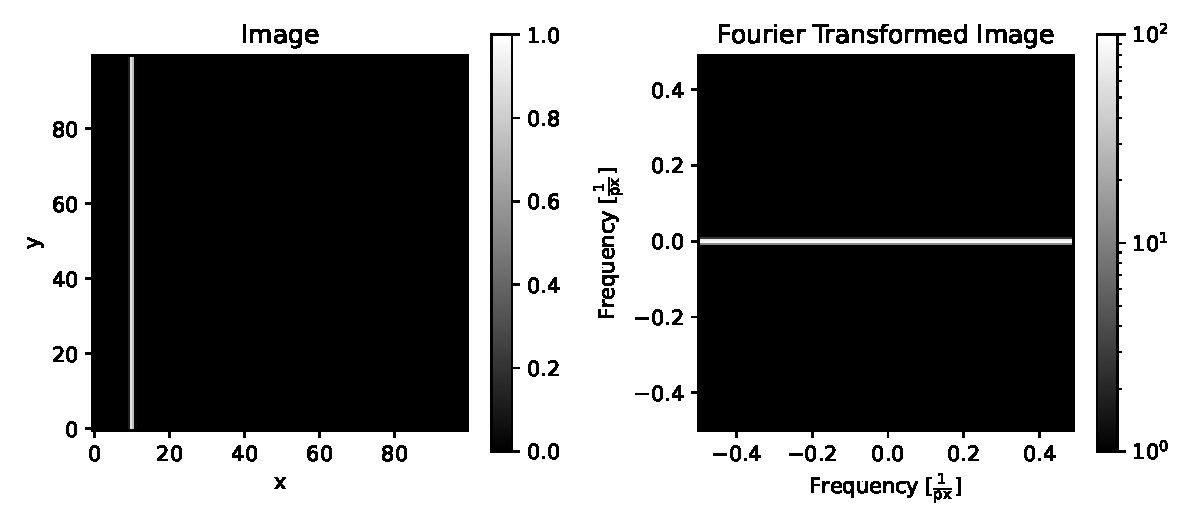
\includegraphics[width=1.0\textwidth]{pics/fft_simulationoneline.pdf}}
		\subfigure[]{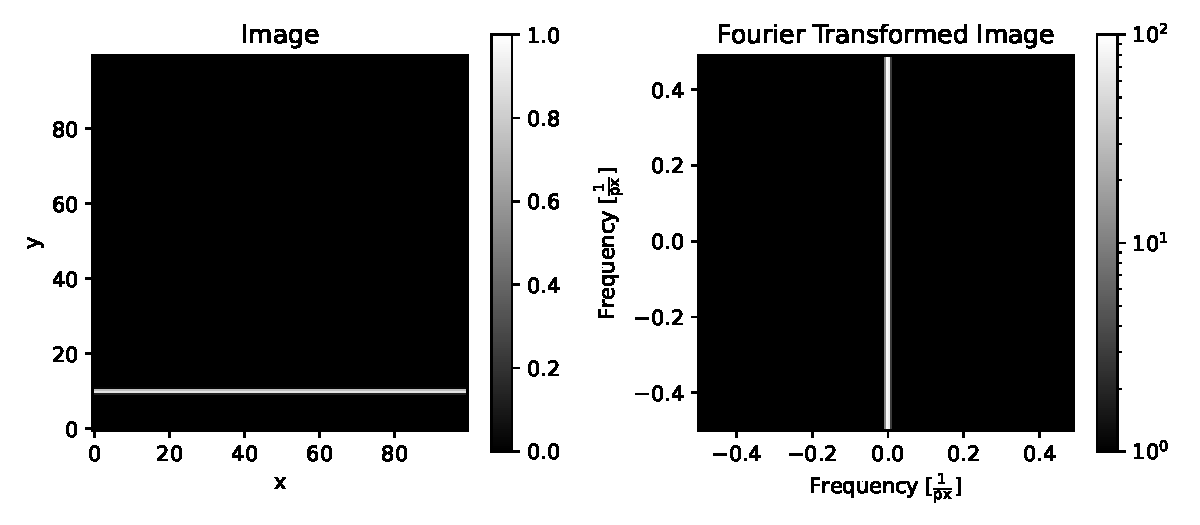
\includegraphics[width=1.0\textwidth]{pics/fft_simulationoneline_horizontal.pdf}}
\caption{The image of a vertical line (a) and of a horizontal line (b) (images on the left side) are transformed to the frequency plane (images on the right side).}
\label{fig:fft_line}
\end{figure}
To explore the frequency plane further we plot the intensity at $y$ frequency equals zero along the $x$ frequency axis (frequency plane of image shown in figure \ref{fig:fft_line} (a)). This describes the periodicity of the image in horizontal direction. As we see in figure \ref{fig:fft_line_cut} the intensity along this axis is constant.
\begin{figure}[H]
	\centering
		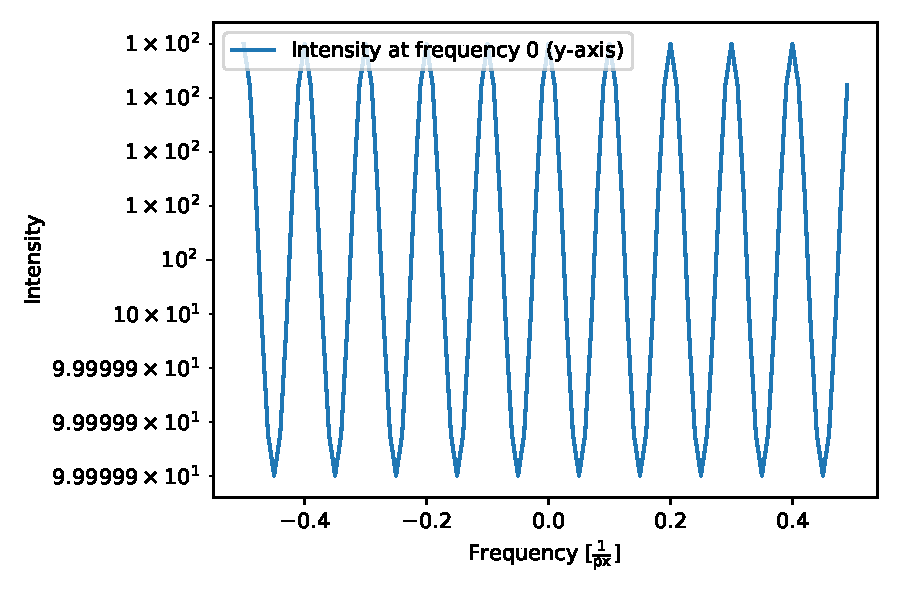
\includegraphics[width=0.8\textwidth]{pics/fft_simulation_cutoneline.pdf}
		\caption{The intensity of the Fourier transformed image in figure \ref{fig:fft_line} (a) at y frequency equals zero.}
		\label{fig:fft_line_cut}
\end{figure}
As a next step we want to find out what happens, if we insert a periodic signal into the image plane in the form of equally spaced lines. Figure \ref{fig:fft_lines} shows an image where there are several vertical lines with a spacing of 20 pixels. As in the case of the single line the image is constant in $y$ direction and so all vertical frequencies are assigned zero. In $x$ direction the lines create a periodic signal with frequency $\frac{1}{20} = 0.05 \frac{1}{\mathrm{px}}$. On the right side of figure \ref{fig:fft_lines} we see the fourier transformation of the image with the equally spaced lines and figure \ref{fig:fft_lines_cut} shows a horizontal cut through the center. We see that only the pixels at $0.05n \frac{1}{\mathrm{px}}$ $\forall n \in \{0, 1, 2, ...\}$ are non-zero.
\begin{figure}[H]
	\centering
		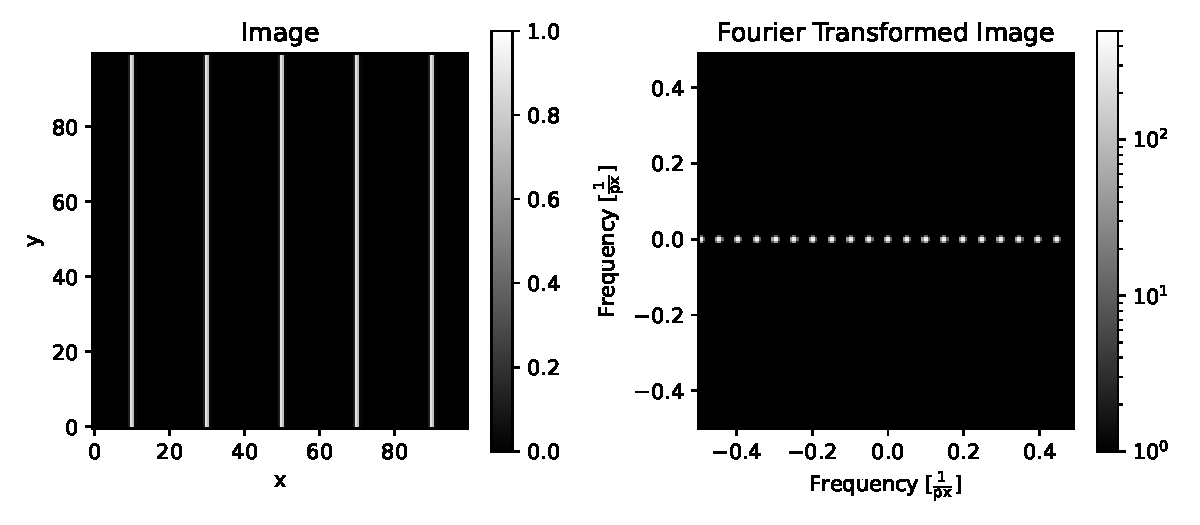
\includegraphics[width=1.0\textwidth]{pics/fft_simulationmorelines.pdf}
		\caption{The image with several equally spaced one pixel thick lines on the left is transformed to the frequency plane, see image on the right.}
		\label{fig:fft_lines}
\end{figure}
\begin{figure}[H]
	\centering
		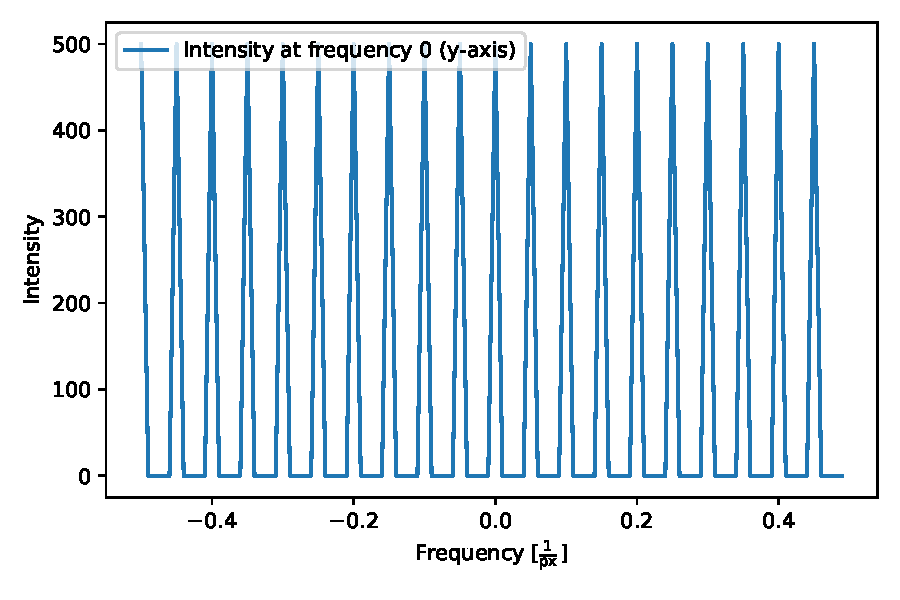
\includegraphics[width=0.8\textwidth]{pics/fft_simulation_cutmorelines.pdf}
		\caption{The intensity of the Fourier transformed image in figure \ref{fig:fft_lines} at y frequency zero.}
		\label{fig:fft_lines_cut}
\end{figure}
In the appendix \ref{almostPeriod} we show, what happens if one line in the periodic image is missing and thus the signal is not completely periodic. We find that the treshold raises up to a higher value.\\
The spiders are not lines, but they have also an expansion into the horizontal, so we are also interested to see the Fourier transform of a single beam. We investigate the image of a beam (stair function) with a width of 10 pixels, placed at $x=10$. Figure \ref{fig:fft_beam} shows the corresponding image and its Fourier transform. As with the lines the only frequencies in the frequency plane with a non-zero value are along the $y=0 \frac{1}{\mathrm{px}}$ frequency axis. Figure \ref{fig:fft_beam_cut} shows this axis in more detail. In contrast to the frequency plane of the line we have a signal which is stronger for central frequencies and decreases slightly for larger frequencies. Additionally we have strong minima at $0.1 n$ $\forall n \in \mathbb{N}$, where the position of the minima is given by one over the width of the beam.
\begin{figure}[H]
	\centering
		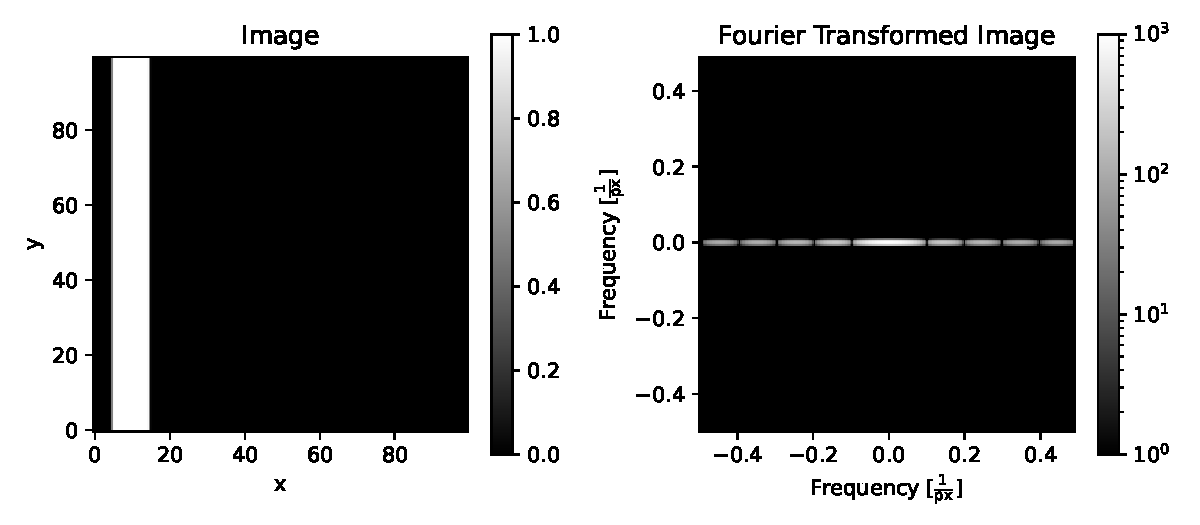
\includegraphics[width=1.0\textwidth]{pics/fft_simulationonebeam.pdf}
		\caption{The image of one 10 pixel thick beam on the left is transformed to the frequency plane, see image on the right.}
		\label{fig:fft_beam}
\end{figure}
\begin{figure}[H]
	\centering
		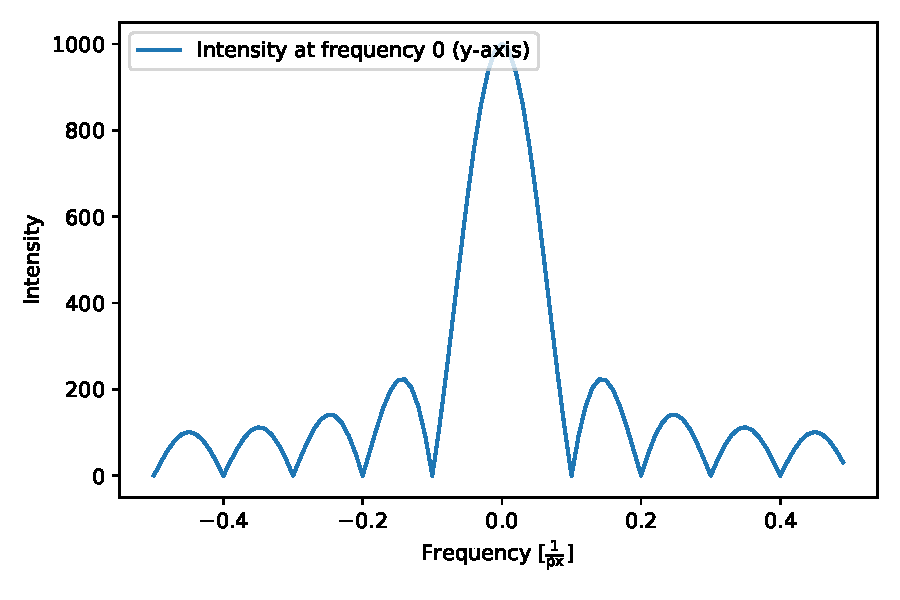
\includegraphics[width=0.8\textwidth]{pics/fft_simulation_cutonebeam.pdf}
		\caption{The intensity of the Fourier transformed image in figure \ref{fig:fft_beam} at y frequency zero.}
		\label{fig:fft_beam_cut}
\end{figure}
As before with the lines we have a look at what happens if we have several of this beams, again equally spaced with a spacing of 20 pixels. We find that this image, lets call it $h(x)$, is a convolution of the image with the equally spaced lines $f(x)$ and the image with the single beam $g(x)$, namely
\begin{equation}
	h(x) = (f * g)(x) = \int_{\mathbb{R}^n} f(\tau)g(x-\tau) \mathrm{d}\tau .
\end{equation}
From the convolution theorem we find that for the Fourier transform it yields:
\begin{equation}
	\mathfrak{F}\{h(x)\} = \mathfrak{F}\{(f * g)(x)\} = (G \cdot F)(\mu),
\end{equation}
where $G(\mu)$ and $F(\mu)$ are the Fourier transforms of $g(x)$ and $f(x)$ \cite{ImageProcessing}. This means that the Fourier transform of the image with the several beams is given by the multiplication of the Fourier transform of the image with the equally spaced lines and the image with the single beam, which can be seen in figure \ref{fig:fft_beams_cut}. Around the center frequency we have some peaks separated by $0.05 \frac{1}{\mathrm{px}} = \frac{1}{20} \frac{1}{\mathrm{px}}$ which describes the separation between the beams of $20$ pixels. This peaks are surrounded by other peaks which are separated by $0.1 \frac{1}{\mathrm{px}} = \frac{1}{10} \frac{1}{\mathrm{px}}$ which describes the width of the beams of $10$ pixels.
\begin{figure}[H]
	\centering
		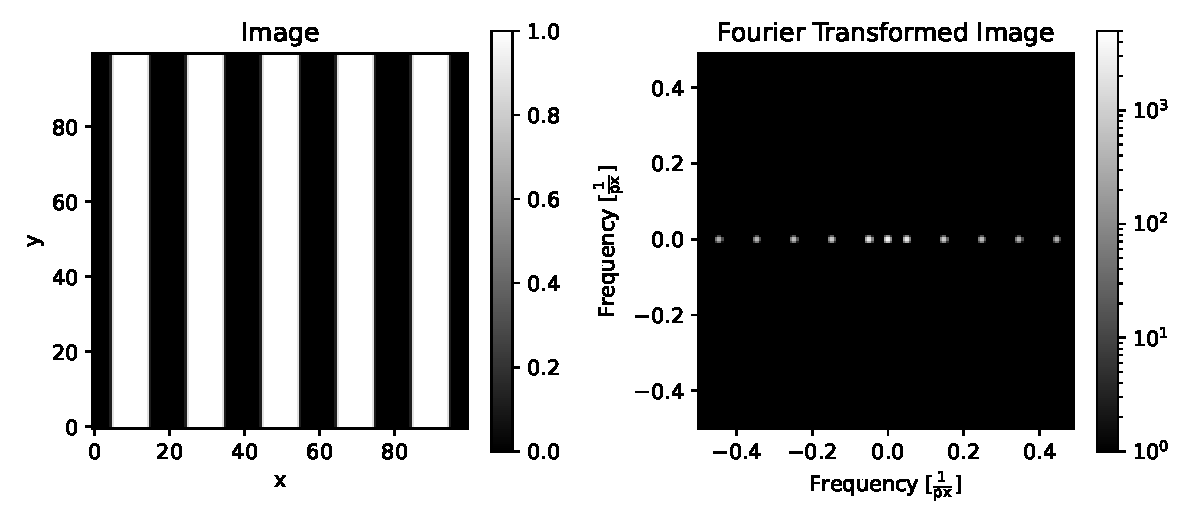
\includegraphics[width=1.0\textwidth]{pics/fft_simulationmorebeams.pdf}
		\caption{The image of several equally spaced 10 pixel thick beam on the left is transformed to the frequency plane, see image on the right.}
		\label{fig:fft_beams}
\end{figure}
\begin{figure}[H]
	\centering
		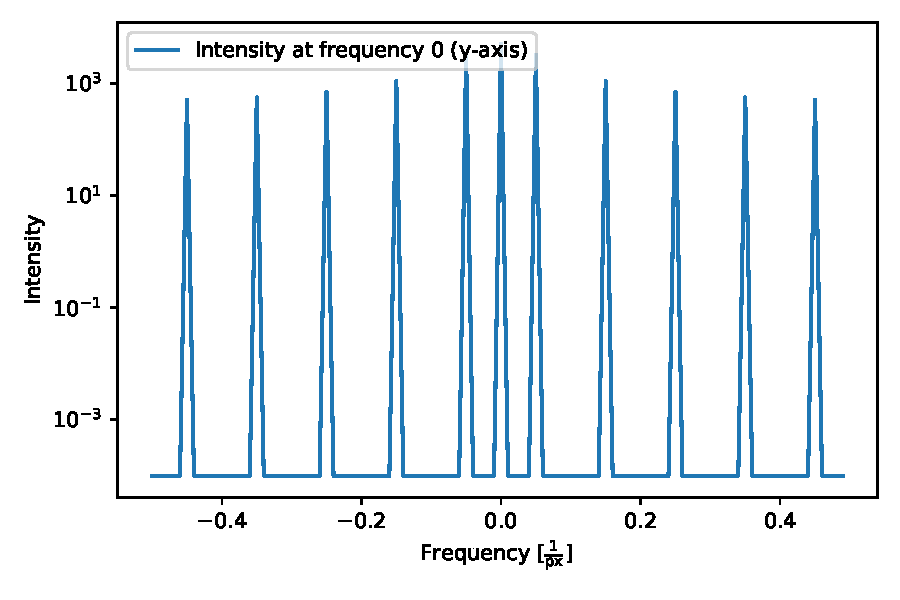
\includegraphics[width=0.8\textwidth]{pics/fft_simulation_cutmorebeams.pdf}
		\caption{The intensity of the Fourier transformed image in figure \ref{fig:fft_beam} at y frequency zero.}
		\label{fig:fft_beams_cut}
\end{figure}

\subsection{Gaussian Beams}
Before we have looked at beams with a stair function shape, but the spiders in our data do not have this stair function shape. In order to have a more realistic approximation we assume the spiders in our simulation to be Gaussian along the radial direction. We calculate the Gaussian profile from 
\begin{equation}
	f(x) = \exp \left(-\frac{(x-\mu)^2}{2 \sigma^2} \right)
\end{equation}
where $\mu$ is the mean (location) and $\sigma$ is the standard deviation (width). \\
Also we change to the image format of the warped image which is not quadratic but rectangular. Four our simulations we choose the radius range 254 to 454 pixels and compare it to the data from HD142527 in this range, which can be seen in figure \ref{fig:warped_254_454}. We have chosen the radius range such that the ghosts lie within it and one of the ghost is in the center of the radius range. So that latter on we can make sure, that we are able to suppress the signal from the spiders without loosing much of the ghosts which we use to simulate a really bright exoplanet. 
\begin{figure}[H]
	\centering
		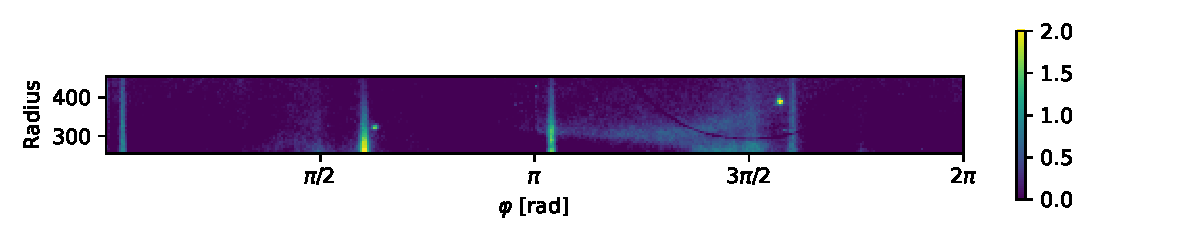
\includegraphics[width=1.0\textwidth]{pics/warped_254_454.pdf}
		\caption{An image of HD142527 which is warped to the $r$-$\varphi$ plane and the radial intensity drop-off is subtracted.}
		\label{fig:warped_254_454}
\end{figure}
Figure \ref{fig:spider_gaussian} shows one of the spiders in a cutout from the image. We can see from the figure that a Gaussian is a good approximation for the shape of the spiders in radial direction.
\begin{figure}[H]
	\centering
		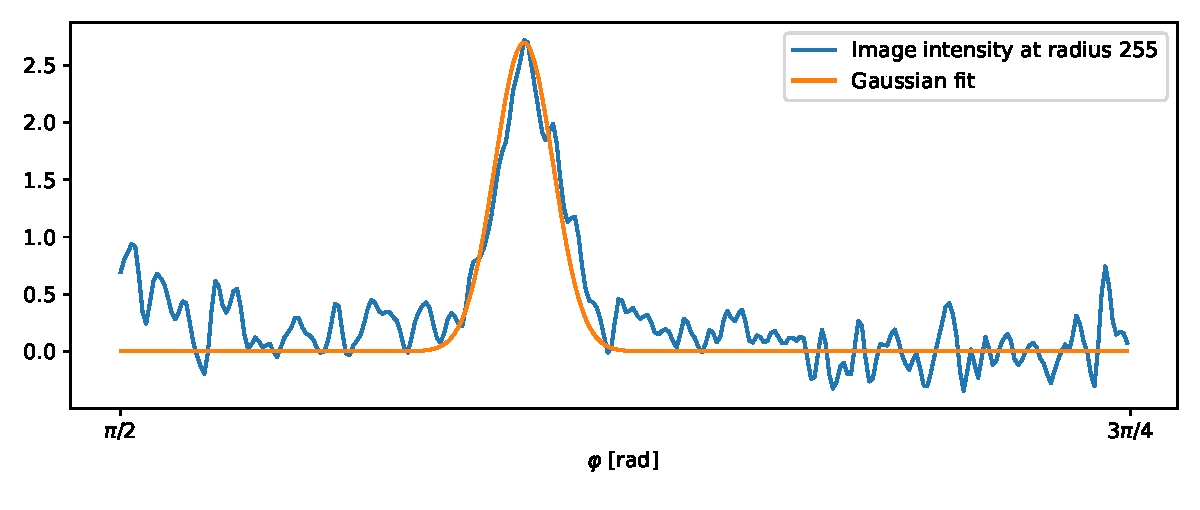
\includegraphics[width=1.0\textwidth]{pics/spyder_gaussian.pdf}
		\caption{A cutout of the image intensity of HD142527 at radius 255, where we see one of the spiders and a Gaussian profile at the same position as the spider is. We can see that the Gaussian is a good approximation for the shape of the spider.}
		\label{fig:spider_gaussian}
\end{figure}
We know that the Fourier transformation of a Gaussian profile is again a Gaussian profile and from the previous subsection we know that the Fourier transform does not depend on the location from the beam, but on the width of it. The spiders in our data all have different widths. In figure \ref{fig:Gauss_diffwidths} we plot four Gaussian profiles with different widths and their Fourier transforms. We see that indeed the Fourier transform of a Gaussian profile is also Gaussian (keep in mind that the plot is logarithmic) and that the width of the Gaussian profile is inverse proportional to the width of its Fourier transform as it already was the case for the stair function beams. Namely that the width of the Fourier transformed Gaussian is $w_{FFT} = \frac{1}{\sigma} \frac{1}{\mathrm{px}}$, where $w_{FFT}$ marks the x-position where the Fourier transformed is again zero. Also the intensity of the Fourier transform decreases with the width of the Gaussian profile, however this effect is rather small in the logarithmic plot. 
\begin{figure}[H]
	\centering
		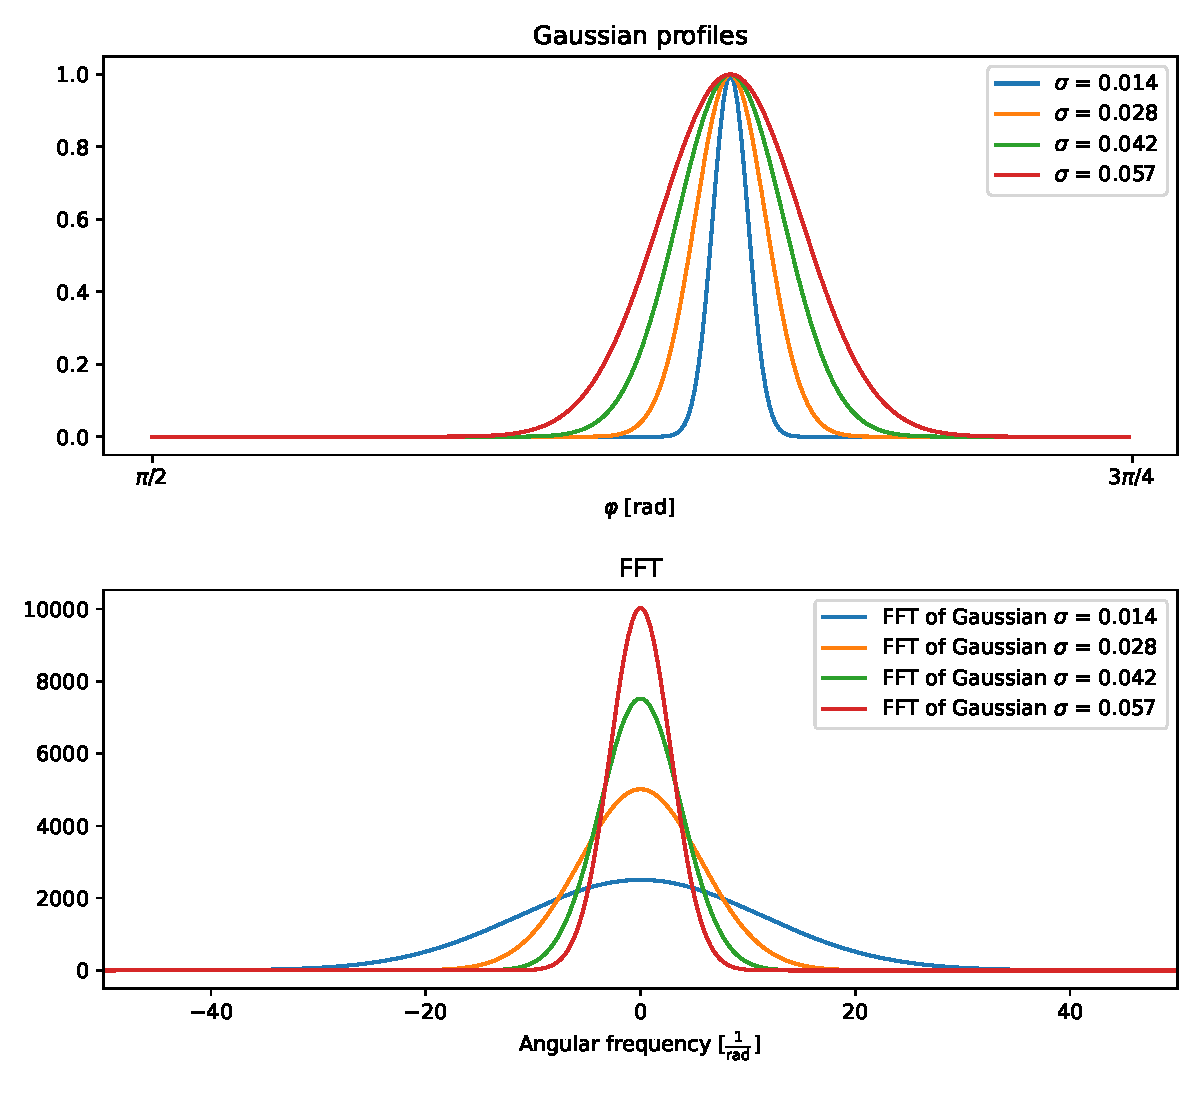
\includegraphics[width=1.0\textwidth]{pics/Gauss_diffwidths.pdf}
		\caption{Gaussian profiles with different widths (top) and the respective Fourier transforms (bottom).}
		\label{fig:Gauss_diffwidths}
\end{figure} 
The VLT telescope produces four spiders which have a 180 degrees symmetry \cite{ESOmanual}. The spiders always have the same distance between each other, but the angular position and width can change from image to image. As a first approximation to this we have a look at four equal Gaussian beams which have the same spacing as in the data and fulfill the 180 degrees symmetry. Figure \ref{fig:Gauss_fourspyders} shows a horizontal cut through this setup and the respective frequency plane. We also plot the Fourier transform of a single Gaussian profile. Due to the linearity of the Fourier transformation we expect the Fourier transformation of the four equal Gaussian to be four times the Fourier transform of the single Gaussian profile. As we see from figure \ref{fig:Gauss_fourspyders}, where also a Fourier transformation of a single Gaussian profile (green line) is contained, this is also the case, but there is a strong oscillation and a beat as well. To understand this oscillation we can use the knowledge which we have gained when we examined the behavior of the beams with stair function shape. There we found that if the image is a convolution of two different functions, then the Fourier transform is the multiplication of the Fourier transform of each function. \\
For a better understanding we have a look at four Gaussian beams which are all separated by 90 degrees, shown in figure \ref{fig:Gauss_fourspyders90}. Here we have as one function the Gaussian profile with a width of $0.034 \mathrm{rad}$,  which if we Fourier transform it produces a Gaussian profile in the frequency plane with a width of $\frac{1}{0.034} = 29.497 \frac{1}{\mathrm{px}}$. The other function in the convolution consists of four lines separated by $\frac{\pi}{2} \mathrm{rad}$, which in the frequency plane corresponds to a large intensity every $\frac{1}{\pi/2} = 0.637 \frac{1}{\mathrm{px}}$ pixel. The multiplication of this two Fourier transformed function results exactly in the image we see in figure \ref{fig:Gauss_fourspyders90}. \\
When we go back to the setting we have in our simulations of the spiders, we do not have equally separated Gaussian profiles. We have the 180 degrees symmetry plus an unknown separation between the neighboring spiders (or Gaussians), this additional information causes an additional convolution which produces the frequency plane we see in figure \ref{fig:Gauss_fourspyders}. 
\begin{figure}[H]
	\centering
		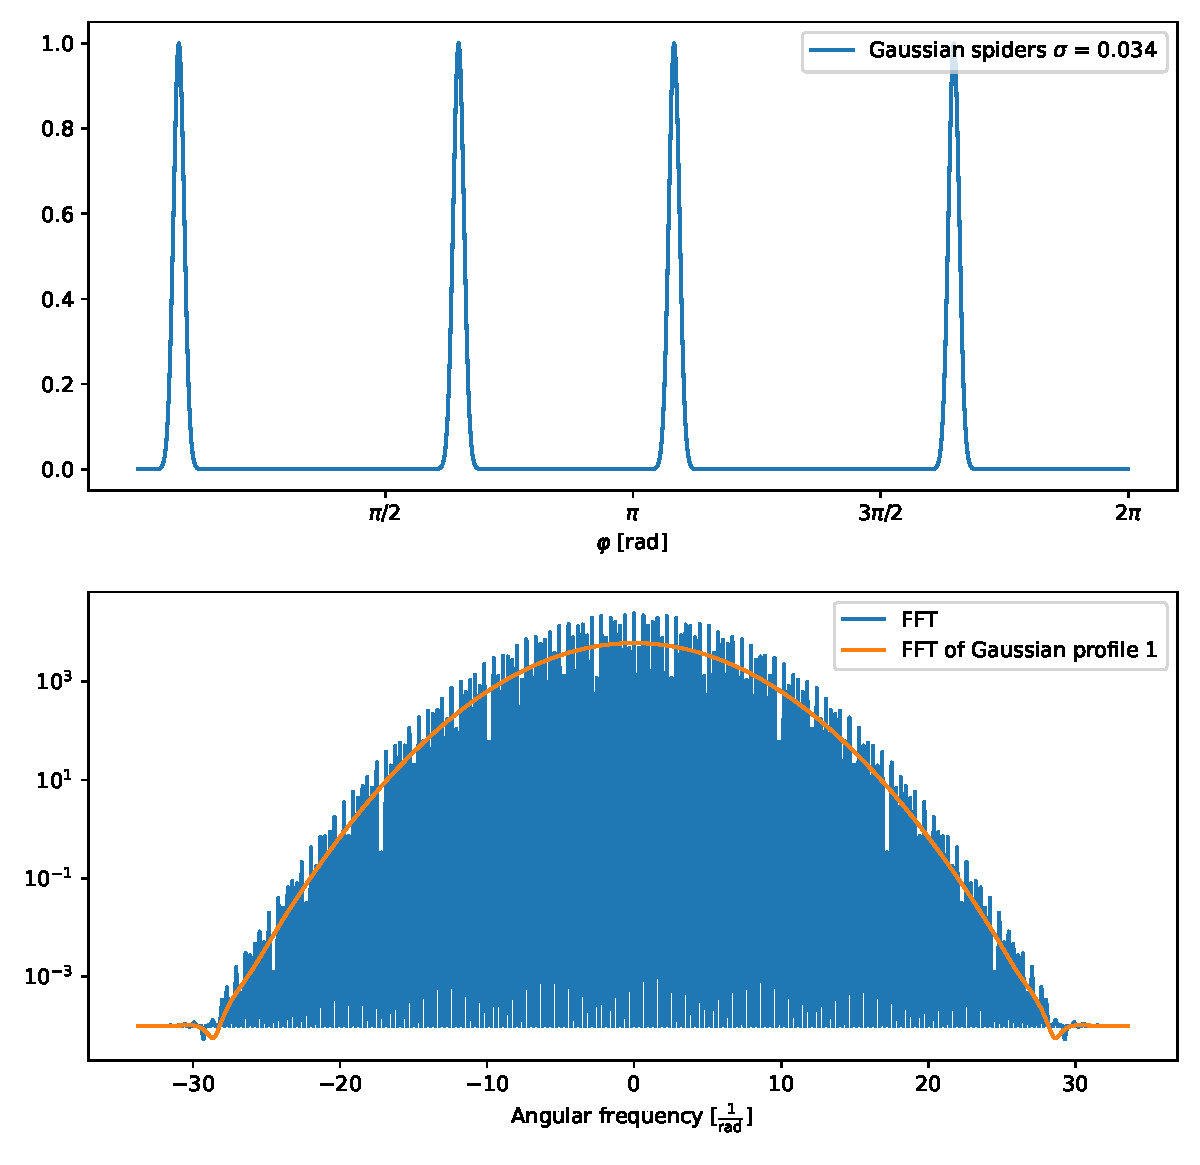
\includegraphics[width=1.0\textwidth]{pics/Gaussian_fourspyders.pdf}
		\caption{The top shows a function with four Gaussian profiles which have a 180 degrees symmetry. The Fourier transform of this is shown in blue in the bottom image. Additionally we plot in green the Fourier transform of a single Gaussian profile.}
		\label{fig:Gauss_fourspyders}
\end{figure} 
\begin{figure}[H]
	\centering
		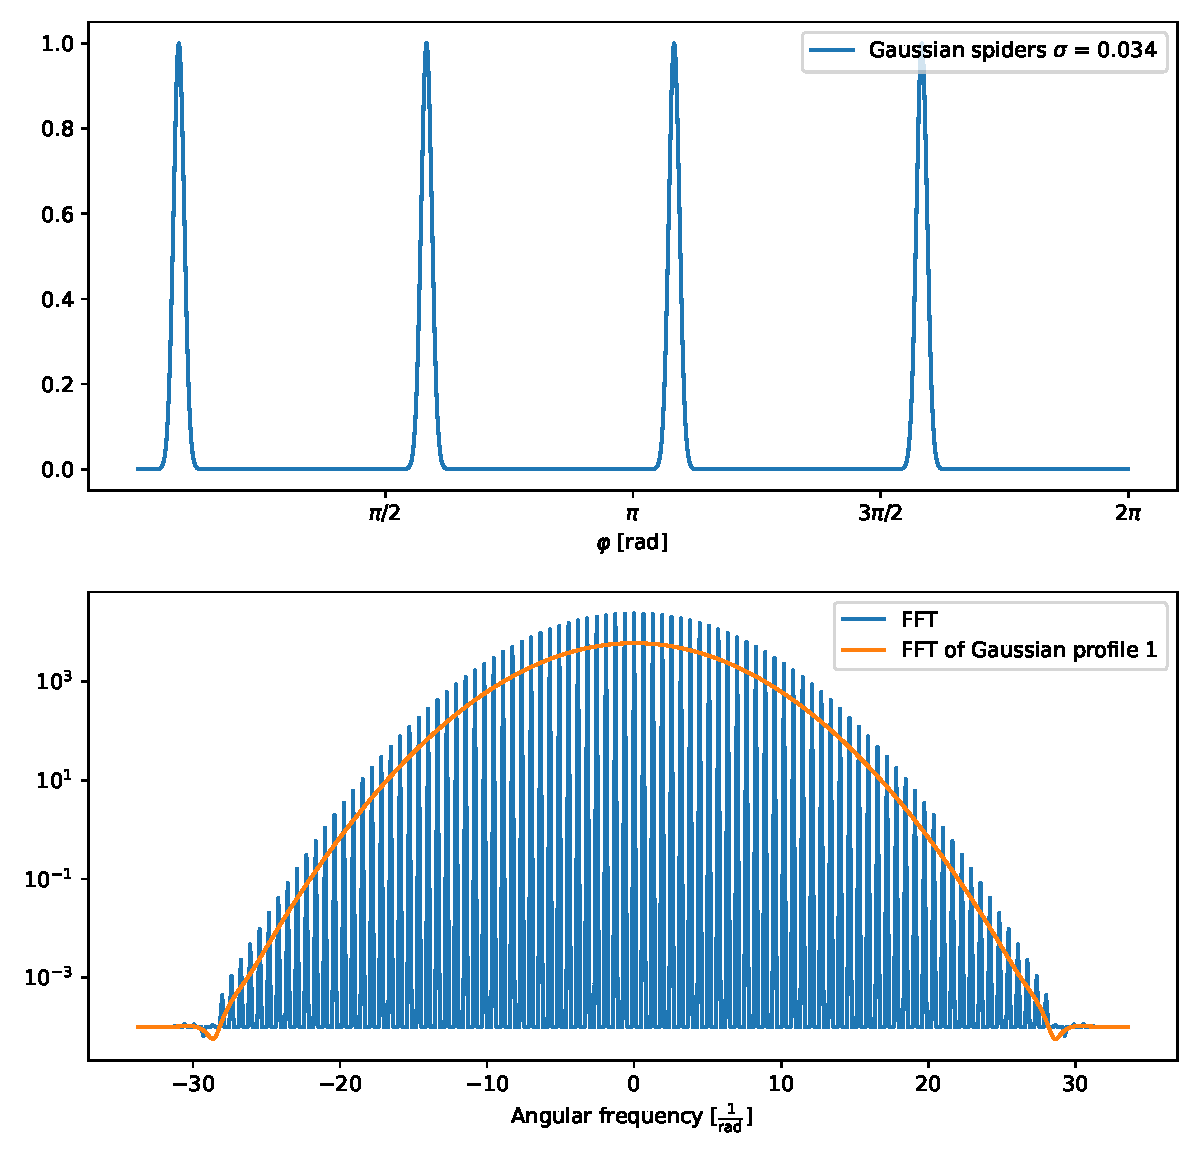
\includegraphics[width=1.0\textwidth]{pics/Gaussian_fourspyders90.pdf}
		\caption{The top shows a function with four Gaussian profiles every 90 degrees. The Fourier transform of this is shown in blue in the bottom image. Additionally we plot in green the Fourier transform of a single Gaussian profile.}
		\label{fig:Gauss_fourspyders90}
\end{figure} 
As a next step we want to include the fact, that the spiders have different widths, see figure \ref{fig:Gaussian_fourdiffspyders}. As we saw from figure \ref{fig:Gauss_diffwidths} the width of the Gaussian mainly influences the width of the Fourier transformed Gaussian and its height. As before we can use the linearity of the Fourier transformation, but now we add up four different Gaussian profiles. Therefore the resulting Fourier transform has the width of the Fourier transform of the thinnest Gaussian profile and the height of the Fourier Transform from the thickest Gaussian profile. We see that the oscillation caused by the convolutions only starts to play a role when the intensity from the respective profile is large enough. 
\begin{figure}[H]
	\centering
		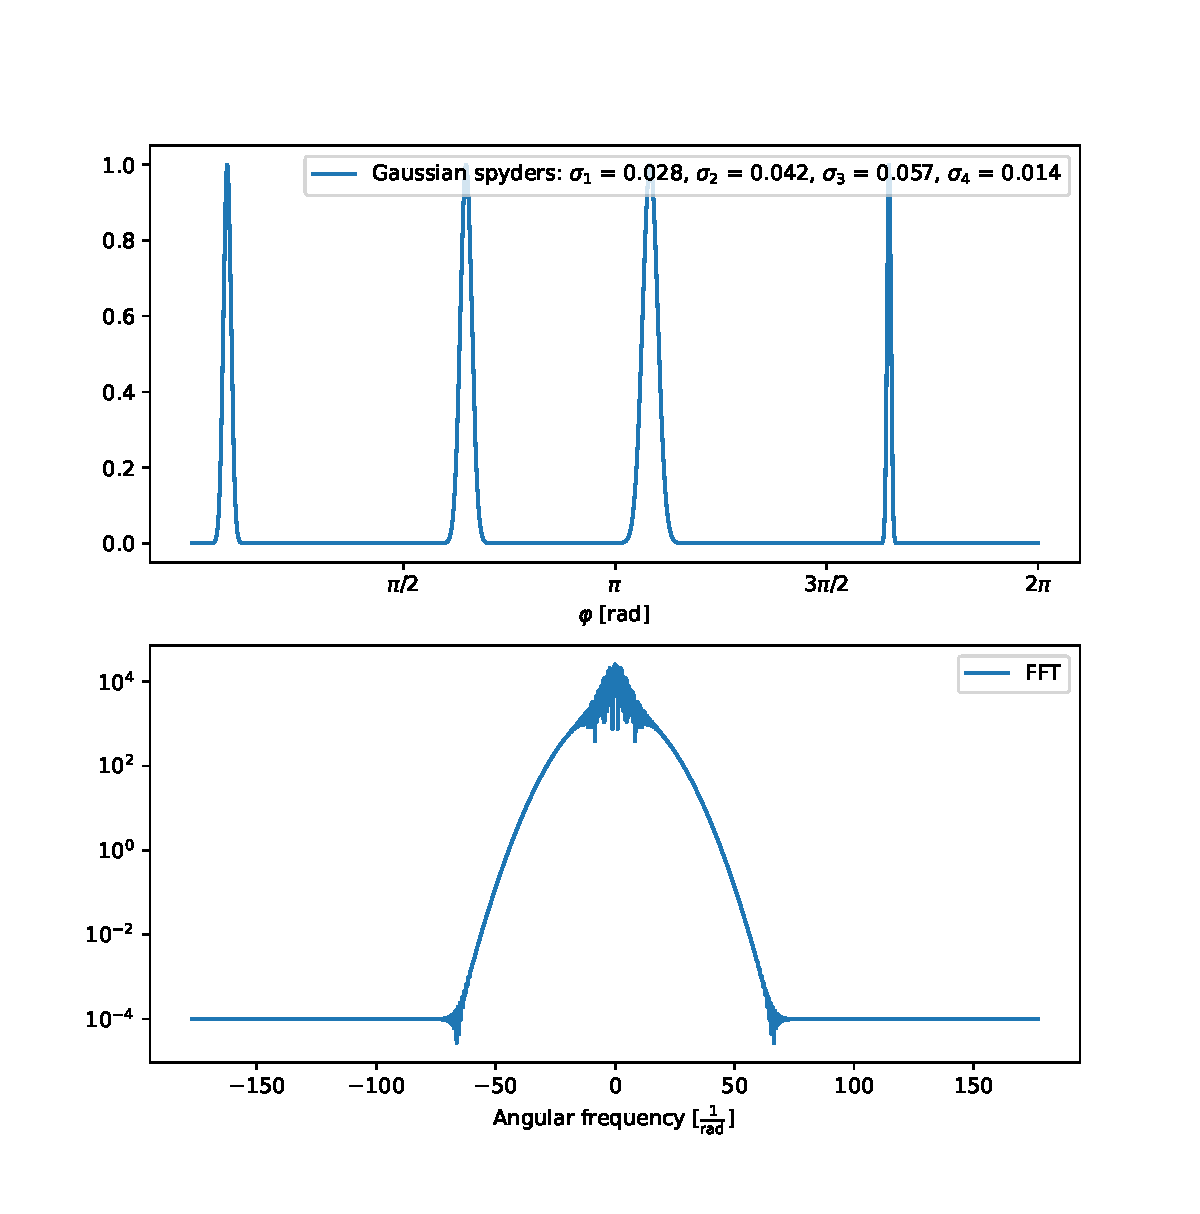
\includegraphics[width=1.0\textwidth]{pics/Gaussian_fourdiffspyders.pdf}
		\caption{The top shows a function with four Gaussian profiles of different widths which have a 180 degrees symmetry. The Fourier transform of this is shown in the bottom image.}
		\label{fig:Gaussian_fourdiffspyders}
\end{figure} 
Finally we also need to take into account that the spiders have different intensities/heights. We look again at the four Gaussian profiles with equal widths which have a 180 degrees symmetry. This time the four Gaussian profiles have different heights as it is shown in the image at the top of figure \ref{fig:Gaussian_fourheightspyders}. Figure \ref{fig:Gaussian_fourheightspyders} also shows the Fourier transform of each profile. We see that the Fourier transform of a profile with a higher intensity also has a higher intensity. When we Fourier transform the whole function which contains all four Gaussian profiles, we get the same Fourier transform as for the one with four equal Gaussian profiles, see figure \ref{fig:Gauss_fourspyders}, but the intensity of the oscillations is smaller and the intensity of the Fourier transform is the summation of the Fourier transform of each profile. 
\begin{figure}[H]
	\centering
		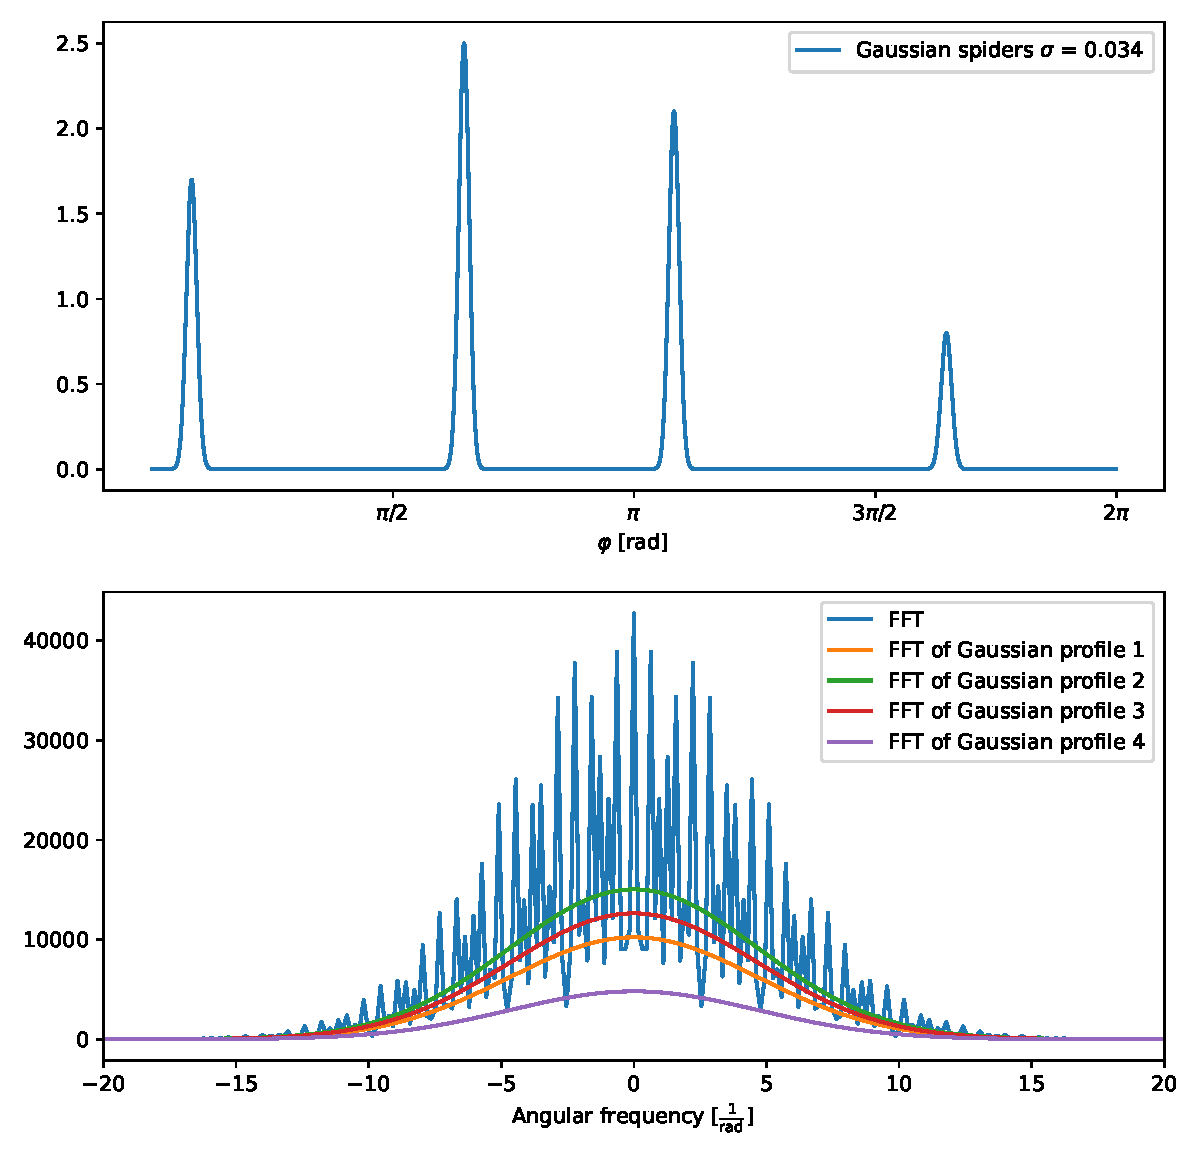
\includegraphics[width=1.0\textwidth]{pics/Gaussian_fourheightspyders.pdf}
		\caption{The top shows a function with four Gaussian profiles of different heights which have a 180 degrees symmetry. The Fourier transform of this is shown in the bottom image.}
		\label{fig:Gaussian_fourheightspyders}
\end{figure}
In conclusion we can say that for four spiders with a 180 degrees symmetry which have different widths and different heights the important frequencies are around the center frequencies. Also the strength of the oscillations are due to the different widths and heights not really strong, so that the intensity could also be approximated by the mean value to cancel out the oscillations.  

\subsection{Spyders}

\subsection{Point-Like Sources}
In order to make sure that we are not going to suppress the signal of point-like sources as exoplanets we need to know how their signal is going to look like in the Fourier space.\\
We investigate the signal of a Gaussian point source and of a point spread function (PSF). A PSF describes how a point source looks like after it has gone through an imaging system \cite{PSFwiki}, which is in our case the VLT telescope with its adaptive optic. In order to simulate the PSF we used the python package AOtools \cite{AOtools}.\\
Figure \ref{fig:PSF_cut_image} shows a cut through the Gaussian and the PSF profile in the image plane. We want to compare the Fourier transformation of the PSF to the one of the Gaussian profile, of which we expect the Fourier transform to be again a Gaussian profile. The image with the PSF and its Fourier transform is shown in figure \ref{fig:PSF_fourier}. Figure \ref{fig:PSF_cut_fourier} shows the Fourier transform of a Gaussian profile and the PSF at radial frequency zero. As expected the Gaussian profile stays Gaussian in the frequency space. The Fourier transform of the PSF produces the same intensity for radial and angular frequency zero, but it decreases slower and has some local maxima. The two local maxima at each side of the global maximum produce a specific pattern which is completely different to what we get from the spiders and might be helpful to extract information about point sources from the frequency plane.  
\begin{figure}[H]
	\centering
		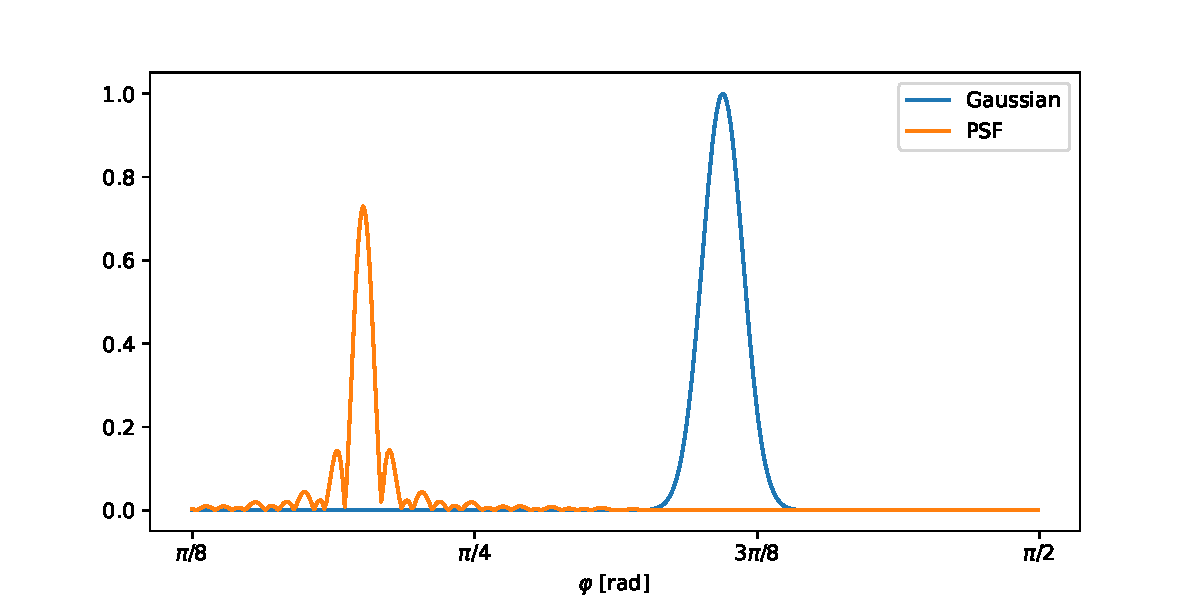
\includegraphics[width=1.0\textwidth]{pics/PSF_cut_image.pdf}
		\caption{A cut through a Gaussian profile and a PSF along the angular direction. Both profiles are rotationally symmetric.}
		\label{fig:PSF_cut_image}
\end{figure}
\begin{figure}[H]
	\centering
		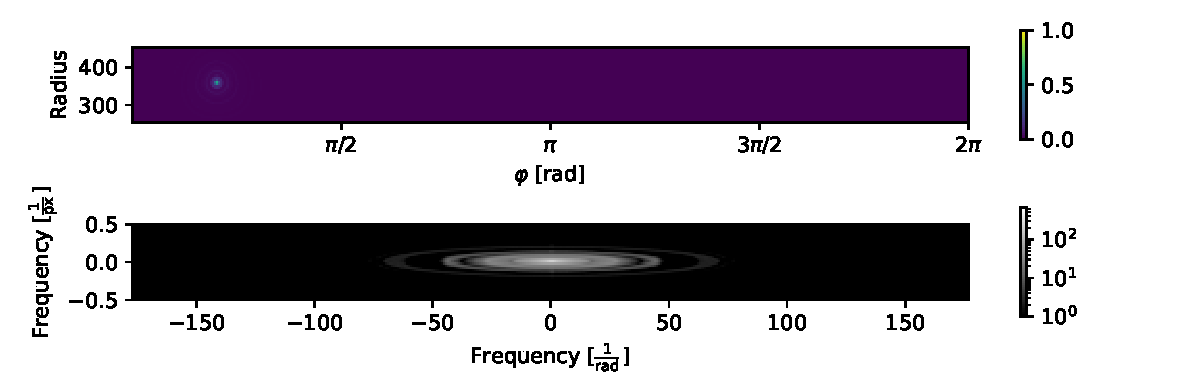
\includegraphics[width=1.0\textwidth]{pics/PSF_fourier.pdf}
		\caption{An image with a PSF (top) is transformed into the frequency space (bottom).}
		\label{fig:PSF_fourier}
\end{figure}
\begin{figure}[H]
	\centering
		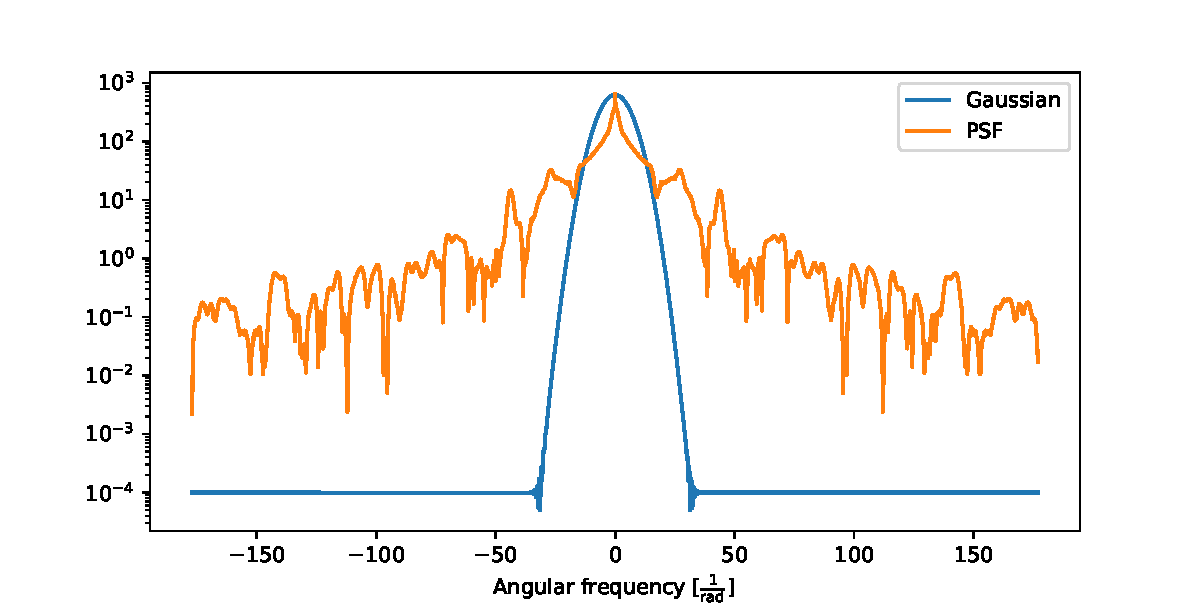
\includegraphics[width=1.0\textwidth]{pics/PSF_cut_fourier.pdf}
		\caption{The Fourier transform of a Gaussian profile and a PSF at radial frequency zero. }
		\label{fig:PSF_cut_fourier}
\end{figure}
